% Options for packages loaded elsewhere
% Options for packages loaded elsewhere
\PassOptionsToPackage{unicode}{hyperref}
\PassOptionsToPackage{hyphens}{url}
\PassOptionsToPackage{dvipsnames,svgnames,x11names}{xcolor}
%
\documentclass[
  letterpaper,
  DIV=11,
  numbers=noendperiod]{scrartcl}
\usepackage{xcolor}
\usepackage{amsmath,amssymb}
\setcounter{secnumdepth}{-\maxdimen} % remove section numbering
\usepackage{iftex}
\ifPDFTeX
  \usepackage[T1]{fontenc}
  \usepackage[utf8]{inputenc}
  \usepackage{textcomp} % provide euro and other symbols
\else % if luatex or xetex
  \usepackage{unicode-math} % this also loads fontspec
  \defaultfontfeatures{Scale=MatchLowercase}
  \defaultfontfeatures[\rmfamily]{Ligatures=TeX,Scale=1}
\fi
\usepackage{lmodern}
\ifPDFTeX\else
  % xetex/luatex font selection
  \setmainfont[]{Times New Roman}
\fi
% Use upquote if available, for straight quotes in verbatim environments
\IfFileExists{upquote.sty}{\usepackage{upquote}}{}
\IfFileExists{microtype.sty}{% use microtype if available
  \usepackage[]{microtype}
  \UseMicrotypeSet[protrusion]{basicmath} % disable protrusion for tt fonts
}{}
\makeatletter
\@ifundefined{KOMAClassName}{% if non-KOMA class
  \IfFileExists{parskip.sty}{%
    \usepackage{parskip}
  }{% else
    \setlength{\parindent}{0pt}
    \setlength{\parskip}{6pt plus 2pt minus 1pt}}
}{% if KOMA class
  \KOMAoptions{parskip=half}}
\makeatother
% Make \paragraph and \subparagraph free-standing
\makeatletter
\ifx\paragraph\undefined\else
  \let\oldparagraph\paragraph
  \renewcommand{\paragraph}{
    \@ifstar
      \xxxParagraphStar
      \xxxParagraphNoStar
  }
  \newcommand{\xxxParagraphStar}[1]{\oldparagraph*{#1}\mbox{}}
  \newcommand{\xxxParagraphNoStar}[1]{\oldparagraph{#1}\mbox{}}
\fi
\ifx\subparagraph\undefined\else
  \let\oldsubparagraph\subparagraph
  \renewcommand{\subparagraph}{
    \@ifstar
      \xxxSubParagraphStar
      \xxxSubParagraphNoStar
  }
  \newcommand{\xxxSubParagraphStar}[1]{\oldsubparagraph*{#1}\mbox{}}
  \newcommand{\xxxSubParagraphNoStar}[1]{\oldsubparagraph{#1}\mbox{}}
\fi
\makeatother


\usepackage{longtable,booktabs,array}
\usepackage{calc} % for calculating minipage widths
% Correct order of tables after \paragraph or \subparagraph
\usepackage{etoolbox}
\makeatletter
\patchcmd\longtable{\par}{\if@noskipsec\mbox{}\fi\par}{}{}
\makeatother
% Allow footnotes in longtable head/foot
\IfFileExists{footnotehyper.sty}{\usepackage{footnotehyper}}{\usepackage{footnote}}
\makesavenoteenv{longtable}
\usepackage{graphicx}
\makeatletter
\newsavebox\pandoc@box
\newcommand*\pandocbounded[1]{% scales image to fit in text height/width
  \sbox\pandoc@box{#1}%
  \Gscale@div\@tempa{\textheight}{\dimexpr\ht\pandoc@box+\dp\pandoc@box\relax}%
  \Gscale@div\@tempb{\linewidth}{\wd\pandoc@box}%
  \ifdim\@tempb\p@<\@tempa\p@\let\@tempa\@tempb\fi% select the smaller of both
  \ifdim\@tempa\p@<\p@\scalebox{\@tempa}{\usebox\pandoc@box}%
  \else\usebox{\pandoc@box}%
  \fi%
}
% Set default figure placement to htbp
\def\fps@figure{htbp}
\makeatother





\setlength{\emergencystretch}{3em} % prevent overfull lines

\providecommand{\tightlist}{%
  \setlength{\itemsep}{0pt}\setlength{\parskip}{0pt}}



 


\usepackage{booktabs}
\usepackage{longtable}
\usepackage{array}
\usepackage{multirow}
\usepackage{wrapfig}
\usepackage{float}
\usepackage{colortbl}
\usepackage{pdflscape}
\usepackage{tabu}
\usepackage{threeparttable}
\usepackage{threeparttablex}
\usepackage[normalem]{ulem}
\usepackage{makecell}
\usepackage{xcolor}
\KOMAoption{captions}{tableheading}
\makeatletter
\@ifpackageloaded{caption}{}{\usepackage{caption}}
\AtBeginDocument{%
\ifdefined\contentsname
  \renewcommand*\contentsname{Table of contents}
\else
  \newcommand\contentsname{Table of contents}
\fi
\ifdefined\listfigurename
  \renewcommand*\listfigurename{List of Figures}
\else
  \newcommand\listfigurename{List of Figures}
\fi
\ifdefined\listtablename
  \renewcommand*\listtablename{List of Tables}
\else
  \newcommand\listtablename{List of Tables}
\fi
\ifdefined\figurename
  \renewcommand*\figurename{Figure}
\else
  \newcommand\figurename{Figure}
\fi
\ifdefined\tablename
  \renewcommand*\tablename{Table}
\else
  \newcommand\tablename{Table}
\fi
}
\@ifpackageloaded{float}{}{\usepackage{float}}
\floatstyle{ruled}
\@ifundefined{c@chapter}{\newfloat{codelisting}{h}{lop}}{\newfloat{codelisting}{h}{lop}[chapter]}
\floatname{codelisting}{Listing}
\newcommand*\listoflistings{\listof{codelisting}{List of Listings}}
\makeatother
\makeatletter
\makeatother
\makeatletter
\@ifpackageloaded{caption}{}{\usepackage{caption}}
\@ifpackageloaded{subcaption}{}{\usepackage{subcaption}}
\makeatother
\usepackage{bookmark}
\IfFileExists{xurl.sty}{\usepackage{xurl}}{} % add URL line breaks if available
\urlstyle{same}
\hypersetup{
  pdftitle={Ejercicios capitulos 4 y 5},
  pdfauthor={Sofia Terra, Santiago Robatto},
  colorlinks=true,
  linkcolor={blue},
  filecolor={Maroon},
  citecolor={Blue},
  urlcolor={Blue},
  pdfcreator={LaTeX via pandoc}}


\title{Ejercicios capitulos 4 y 5}
\author{Sofia Terra, Santiago Robatto}
\date{2025-09-16}
\begin{document}
\maketitle


\subsection{Ejercicio 4.19}\label{ejercicio-4.19}

Lo primero que se realizó fue cargar la data y filtrarla por el año de
interés (1980).

\begin{verbatim}
 binary  n   percent
   FAIL 10 0.7142857
   PASS  4 0.2857143
  Total 14 1.0000000
\end{verbatim}

Generamos el grafico de prior, verosimilitud y posterior con plot beta
binomial

\pandocbounded{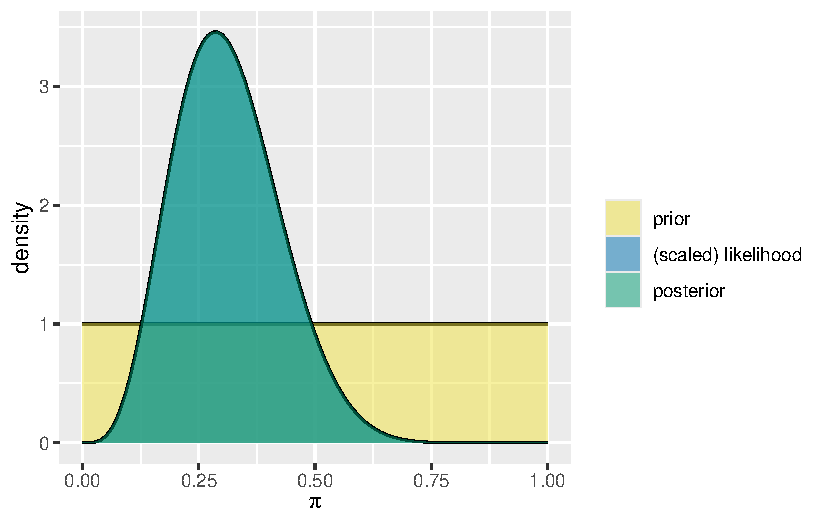
\includegraphics[keepaspectratio]{prueba_files/figure-pdf/unnamed-chunk-4-1.pdf}}

Se observa que la verosimilitud es igual al posterior. Esto ocurre
porque el prior es una beta (1,1) que es uniforme en el recorrido.
Interpretando esto de una manera bayesiana, signfiica que no aporta nada
de informacion. Se utiliza para repersentar neutralidad absoltua.
Siempre que partimos de una beta con tales parametros, la verosimilud
sera igual al posterior.

El posterior alcanza su moda entorno a 0.25 y deja prácticamente con
probabilidad 0 alos valores superiores a 0.5. Esto nos da indicios que
la varianza será considerablemente baja.

Para el \textbf{Cálculo teórico de la esperanza y modo} utilizaremos el
calculo del posterior del modelo beta binomial, que sabemos que
distribuye Beta (\(\alpha\)+y,\(\beta\)+n-y).

Dada dicha distribución, sabemos que la esperanza del posterior será:

\[
\mathbb{E}[\pi] = \frac{\alpha + y}{\alpha + y + \beta + n - y} =  \frac{\alpha + y}{\alpha  + \beta + n }= \frac{1+4}{1+1+14}=\frac{5}{16}= 0.3125
\]

\begin{longtable}[t]{lrrrrrr}
\caption{\label{tab:unnamed-chunk-6}Medidas de resumen beta-binomial(1, 1, 4, 14)}\\
\toprule
model & alpha & beta & mean & mode & var & sd\\
\midrule
prior & 1 & 1 & 0.5000 & NaN & 0.0833 & 0.2887\\
posterior & 5 & 11 & 0.3125 & 0.2857 & 0.0126 & 0.1124\\
\bottomrule
\end{longtable}

De esta manera comprobamos que la Esperanza hallada de manera teórica es
igual a la esperanza hallada por la función summarize.

Se refuerza la información que vimos en el gráifco del prior y
posterior. Si bien comentamos que la moda del posterior estaba entorno a
0.25, ahora visualizamos que es exactamente 0.2857. Por otro lado se
reafirma la baja varianza que comentamos.

Finalemnte, es correcto que no exista el modo del prior, dado que es una
beta(1,1) y esta perfectamente equidistribuida.

\subsubsection{Parte dos: Calculo para
1990}\label{parte-dos-calculo-para-1990}

Busqueda de la informacion para 1990 (Verosimilitud)

\begin{verbatim}
 binary  n percent
   FAIL  9     0.6
   PASS  6     0.4
  Total 15     1.0
\end{verbatim}

Partimos del posterior anterior que ya sabemos como distribuye gracias a
la formula del posterior en el modelo beta binomial y cargamos la
verosimilitud buscada en el paso anterior. Dicho ``posterior'' se
convirtio en nuestro nuevo prior y se agrega una nueva verosimilitud.

\pandocbounded{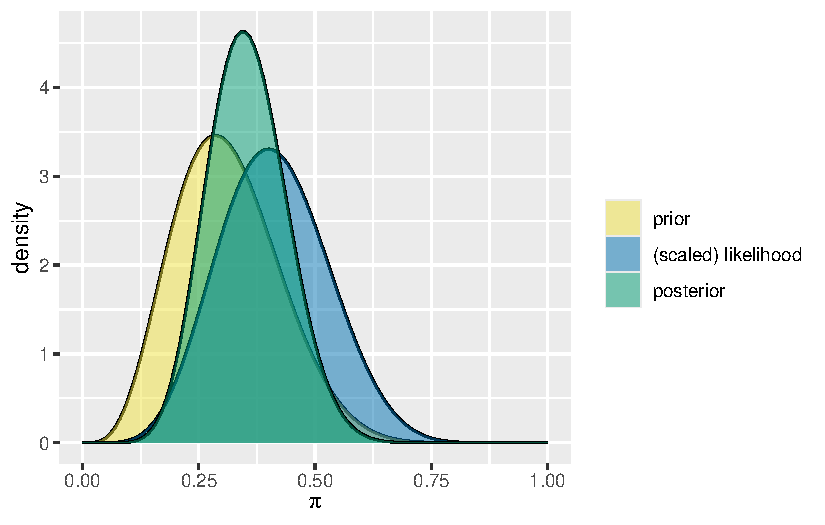
\includegraphics[keepaspectratio]{prueba_files/figure-pdf/unnamed-chunk-8-1.pdf}}

Se observa que el psoterior está en un punto medio entre priory
verosimiitud. Entendemos que esto es correcto dado que el n dado no es
lo suficientemente grande para volcar los datos hacia la verosimilitud,
y además prior y verosimilitud son igual de concentrados entorno a un
valor, ninguno es mucho más disperso ni concentrado que el otro.

\begin{longtable}[t]{lrrrrrr}
\caption{\label{tab:unnamed-chunk-10}Medidas de resumen beta-binomial(5, 11, 6, 15)}\\
\toprule
model & alpha & beta & mean & mode & var & sd\\
\midrule
prior & 5 & 11 & 0.3125 & 0.2857 & 0.0126 & 0.1124\\
posterior & 11 & 20 & 0.3548 & 0.3448 & 0.0072 & 0.0846\\
\bottomrule
\end{longtable}

\subsubsection{Parte 3: Año 2000}\label{parte-3-auxf1o-2000}

Nuestro nuevo prior distribuira Beta(11, 20)

\begin{verbatim}
 binary  n   percent
   FAIL 34 0.5396825
   PASS 29 0.4603175
  Total 63 1.0000000
\end{verbatim}

\pandocbounded{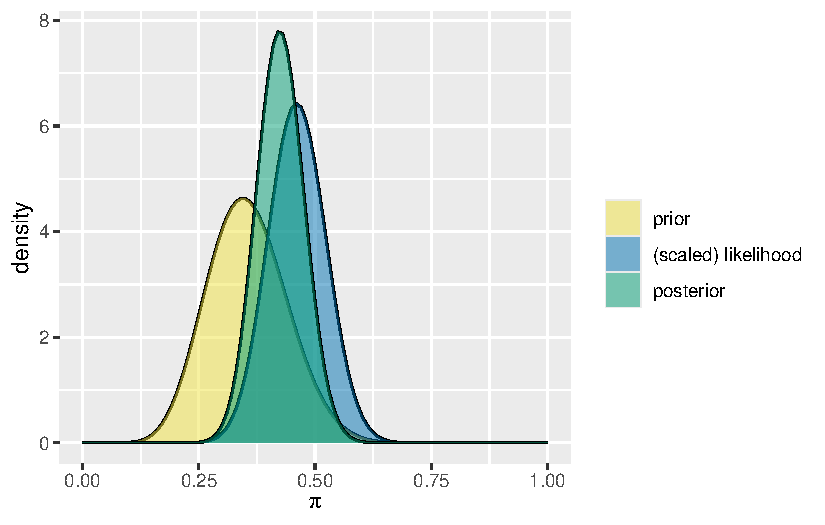
\includegraphics[keepaspectratio]{prueba_files/figure-pdf/unnamed-chunk-12-1.pdf}}

\begin{longtable}[t]{lrrrrrr}
\caption{\label{tab:unnamed-chunk-14}Medidas de resumen beta-binomial(11, 20, 29, 63)}\\
\toprule
model & alpha & beta & mean & mode & var & sd\\
\midrule
prior & 11 & 20 & 0.3548 & 0.3448 & 0.0072 & 0.0846\\
posterior & 40 & 54 & 0.4255 & 0.4239 & 0.0026 & 0.0507\\
\bottomrule
\end{longtable}

\subsubsection{Parte 4: Calculo de
Jenna}\label{parte-4-calculo-de-jenna}

\begin{verbatim}
 binary  n  percent
   FAIL 53 0.576087
   PASS 39 0.423913
  Total 92 1.000000
\end{verbatim}

\pandocbounded{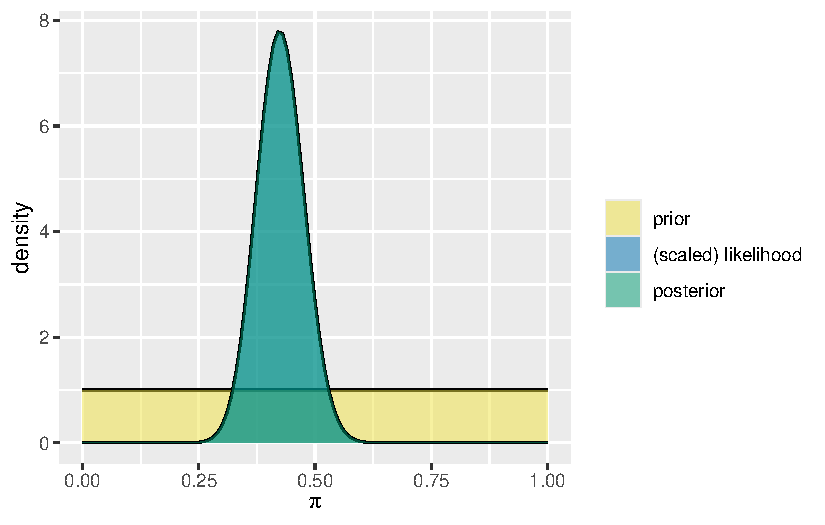
\includegraphics[keepaspectratio]{prueba_files/figure-pdf/unnamed-chunk-16-1.pdf}}

\begin{longtable}[t]{lrrrrrr}
\caption{\label{tab:unnamed-chunk-18}Medidas de resumen beta-binomial(1, 1, 39, 92)}\\
\toprule
model & alpha & beta & mean & mode & var & sd\\
\midrule
prior & 1 & 1 & 0.5000 & NaN & 0.0833 & 0.2887\\
posterior & 40 & 54 & 0.4255 & 0.4239 & 0.0026 & 0.0507\\
\bottomrule
\end{longtable}

Se observa que Jenna llega a la misma posterior que John; probando que
no importa el orden en el que mires la informacion, se llegara a los
mismos resultados. John realiza su analisis en tres dias (pasos),
mientras que Jenna solo en uno. Pero al partir del mismo prior
(Beta(1,1)) y utilizar las mismas muestras, llegan a los mismos
posteriors.

Esta propiedad es denominada \textbf{propiedad de consistencia} o
tambien \textbf{acumulacion secuencial} y como comentamos anteriormente
permite actualizar de una sola vez o en ``capas''.

\subsection{Ejercicio 5.7: Womens world
cup}\label{ejercicio-5.7-womens-world-cup}

Utilizaremos plot\_gamma (1, 0.25) dado que es el prior dado.

\pandocbounded{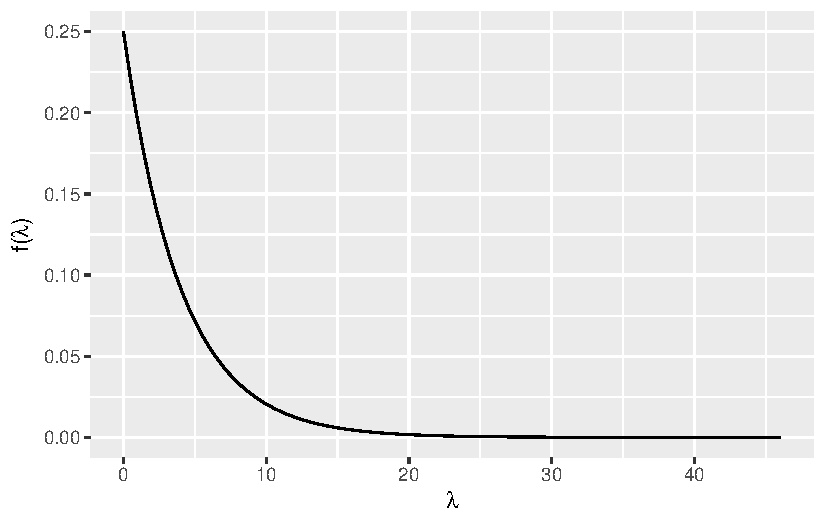
\includegraphics[keepaspectratio]{prueba_files/figure-pdf/unnamed-chunk-19-1.pdf}}

Se observa que \(\lambda\) es decreciente y parte desde cero, con
asimetria a la derecha. Es sumamente coherente con el contexto de que
\(\lambda\) representa la cantidad de goles promedio, seria extrano que
20 tenga probabilidad alta, por ejemplo. Sugiere que no habra goles en
la mayoria de partidos.

\subsubsection{Parte 2: Yi para modelo
Poisson}\label{parte-2-yi-para-modelo-poisson}

Se utiliza el modelo Poisson para representar a Y dado que este es util
para los conteos. Y es una variable aleatoria para representar los
goles.

Cada Yi es una observacion, es decir los goles de cada partido puntual.
Por otro lado \(\lambda\) representa la tasa media de ocurrencia, osea,
la cantidad promedio de goles por partido.

\subsubsection{Parte 3: Total de goles por
partido}\label{parte-3-total-de-goles-por-partido}

\pandocbounded{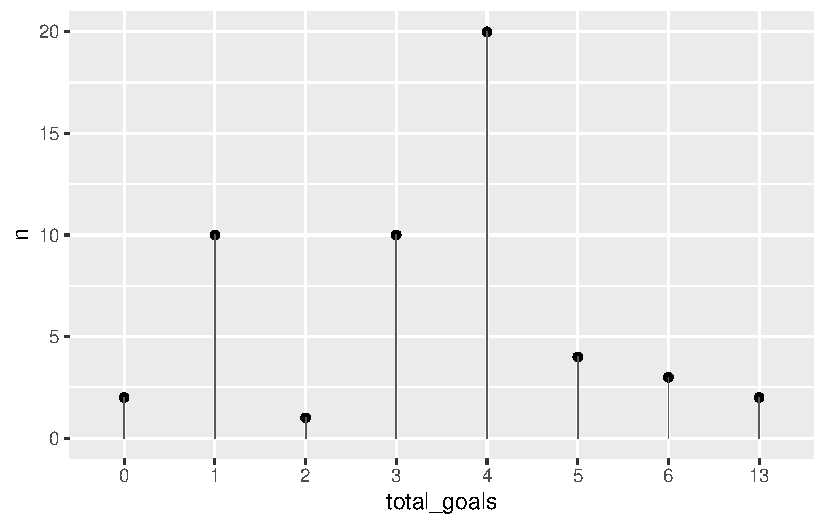
\includegraphics[keepaspectratio]{prueba_files/figure-pdf/unnamed-chunk-22-1.pdf}}

Se observan la cantidad de goles por partido y cuantas veces se repite
ese resutado, es decir la frecuencia para cada resultado.

Para poder graficar el posterior y la verosimilitud necesitaremos
calcular el total de goles que se convirtieron y el total de partidos.
Este ultimo se observa que es 52 en wwc\_2019\_matches.

Para calcular el total de goles, debemos multriplcar la frecuencia de
cada resultado por el total de goles de ese resultad yluego sumarlo.

Removeremos el valor NA que generamos antes al utilizar as.numeric
(generamos NA el total, que NO interesa graficarlo y alteraria la
consistencia de nuestros datos)

\pandocbounded{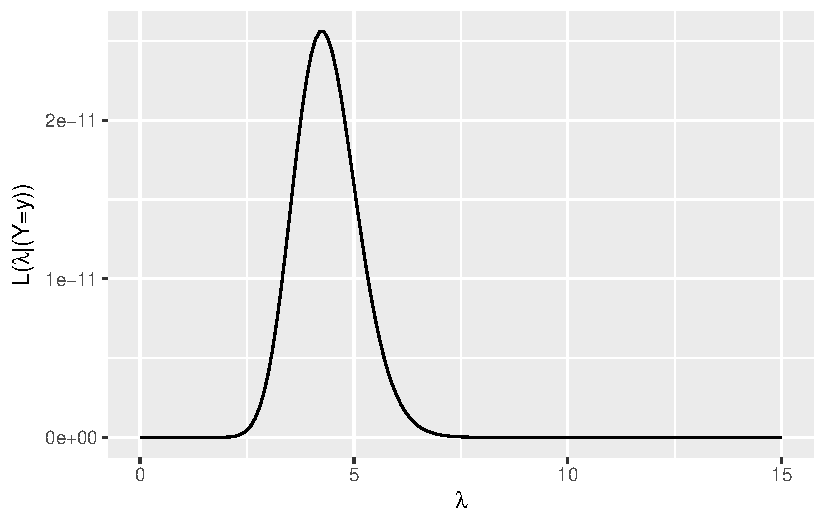
\includegraphics[keepaspectratio]{prueba_files/figure-pdf/unnamed-chunk-24-1.pdf}}

Se observa que los valores mas verosimiles de \(\lambda\) rondan entre 3
y 5 goles de media por partido. Es una likelihood muy agresiva, en el
sentido de que asigna probabilidad practicamente nula a 0 y 1 gol.

\subsubsection{Grafico del posterior}\label{grafico-del-posterior}

Ahora interesa calcular el posterior. Para ello utilizaremos la funcion
plot\_gamma\_poisson.

\pandocbounded{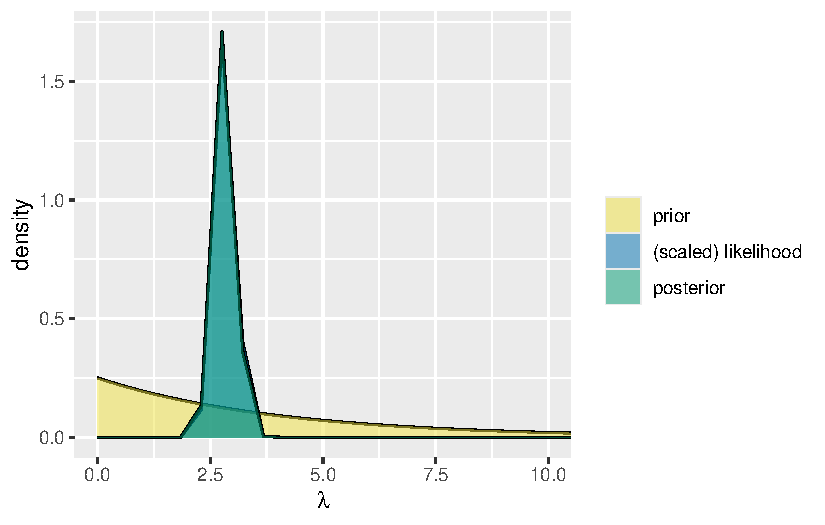
\includegraphics[keepaspectratio]{prueba_files/figure-pdf/unnamed-chunk-25-1.pdf}}

En este caso, el posterior y la likelihood son practicamente iguales.
Recien al hacer zoom encontramos una pequena diferencia:

\begin{figure}[H]

{\centering 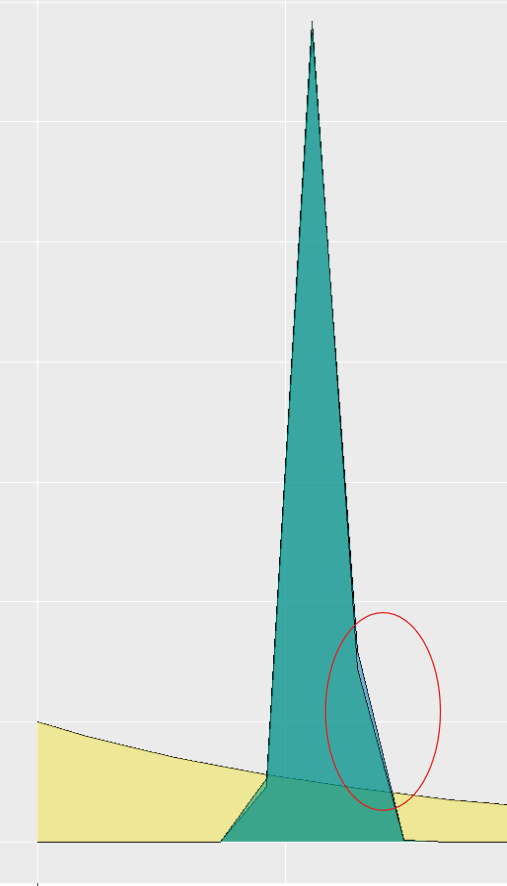
\includegraphics[width=0.6\linewidth,height=0.4\textheight]{a.png}

}

\caption{Diferencia entre Posterior y likelihood}

\end{figure}%

Pensamos que esto ocurre por varios motivos: Tenemos un n
considerablemente grande (52), la funcion de verosimilitud esta
sumamente concentrada entorno a un valor y el prior no esta tan
concentrado, sino que es mas disperso.

De esta manera, hay un cambio radical en nuestro entendimiento de la
media de goles por partido. De pasar de pensar que la media podia ser 0,
1 o 2, pasamos a poder afirmar que la media de goles por partido estara
en el entorno de 3.

\#Ejercicio 5.12: Control brains

Aclaracion: Cuando la letra del ejercicio plantea ``control subjects who
have not been diagnosed with a concussion'', entendemos que refiere al
grupo denominado control, pero puede haber habido un error de
interpretacion.

Primero procederemos con cargar la data y filtrarla para el grupo de
control.

\begin{verbatim}
  mean(volume)
1       7.6026
\end{verbatim}

El promedio de los sujetos que no tuvieron contusiones es de 7.6026 cm3
en una muestra de 25 personas.

\pandocbounded{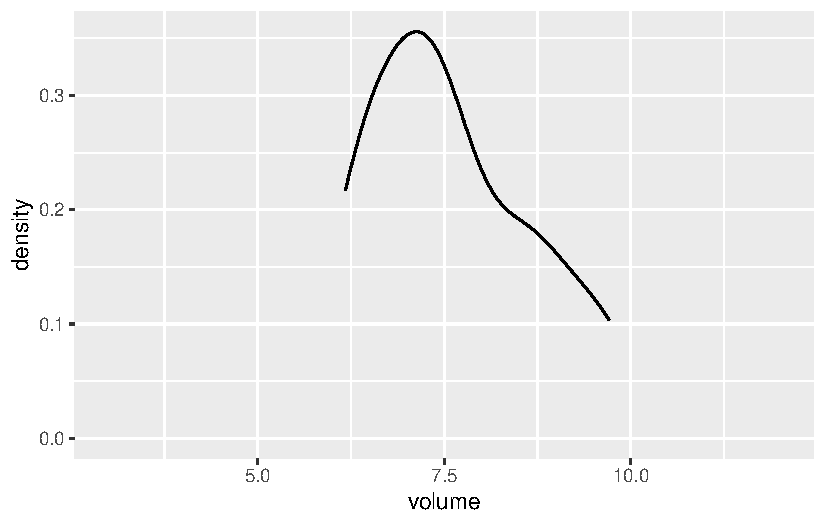
\includegraphics[keepaspectratio]{prueba_files/figure-pdf/unnamed-chunk-28-1.pdf}}

Se observa que los valores van desde 6.175 hasta 9.71 y alcanzan el
maximo de densidad entorno a 7.3, que es levemente menor al promedio
(7.6026).

\pandocbounded{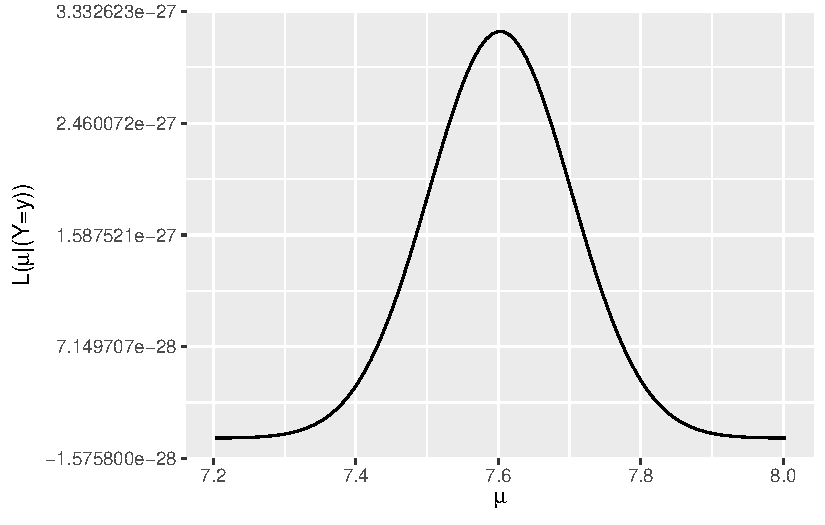
\includegraphics[keepaspectratio]{prueba_files/figure-pdf/unnamed-chunk-29-1.pdf}}

De esta manera se visualiza la verosimilitud de u. Los datos reflejan
que la media, que calculamos anteriormente es el valor mas probable.

\subsubsection{Calculo del posterior}\label{calculo-del-posterior}

Ya tenemos todo lo necesario para identificar el posterior: El prior
tiene media θ=6.5 y τ=0.4 La muestra de los que no tuvieron contusion
tiene media y=7.6026 y asumimos desvio conocido, pero por letra del
ejercicio σ=0.5.

Sabemos que el Modelo Normal-Normal distribuye de la siguiente manera:

\[
\begin{aligned}
Y_i|\mu &\stackrel{ind}{\sim} N(\mu, \sigma^2) \\
\mu &\sim N(\theta, \tau^2)
\end{aligned}
\]

\[
\mu|\vec{y} \sim N\left(\theta\frac{\sigma^2}{n\tau^2 + \sigma^2} + \bar{y}\frac{n\tau^2}{n\tau^2 + \sigma^2}, \frac{\tau^2\sigma^2}{n\tau^2 + \sigma^2}\right)
\]

Por lo tanto, sustituyendo los valores que obtuvimos llegammos a que el
modelo bayesiano conjugado Normal-Normal es el siguiente:

\[
\mu|\vec{y} \sim N\left(6.5\frac{0.5^2}{25*0.4^2 + 0.5^2} + \bar{7.6026}\frac{25*0.4^2}{25*0.4^2 + 0.5^2}, \frac{0.4^20.5^2}{25*0.4^2 + 0.5^2}\right)
\] Entonces:

\[
\mu|\vec{y} \sim N(7.538, \ 0.0094)
\]

El grafico de nuestra distriubucion queda de la forma:

\pandocbounded{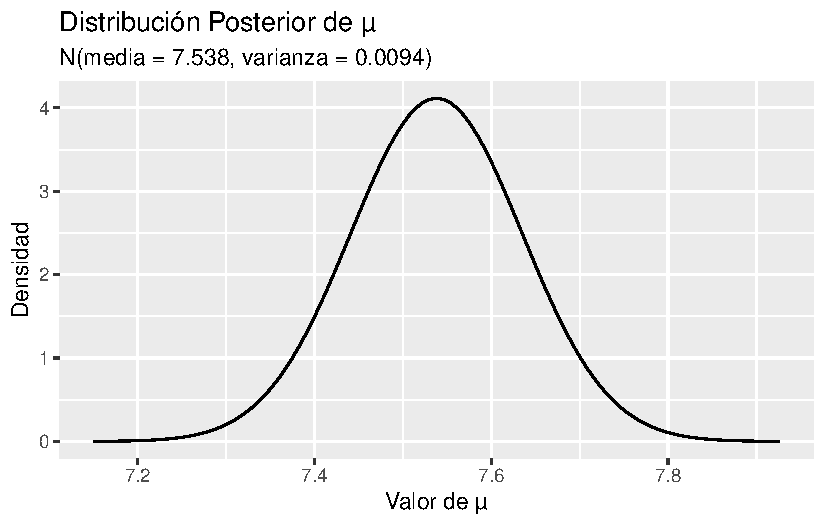
\includegraphics[keepaspectratio]{prueba_files/figure-pdf/unnamed-chunk-30-1.pdf}}

\subsubsection{Parte 3: Plot del prior, verosimilitud y
posterior}\label{parte-3-plot-del-prior-verosimilitud-y-posterior}

\pandocbounded{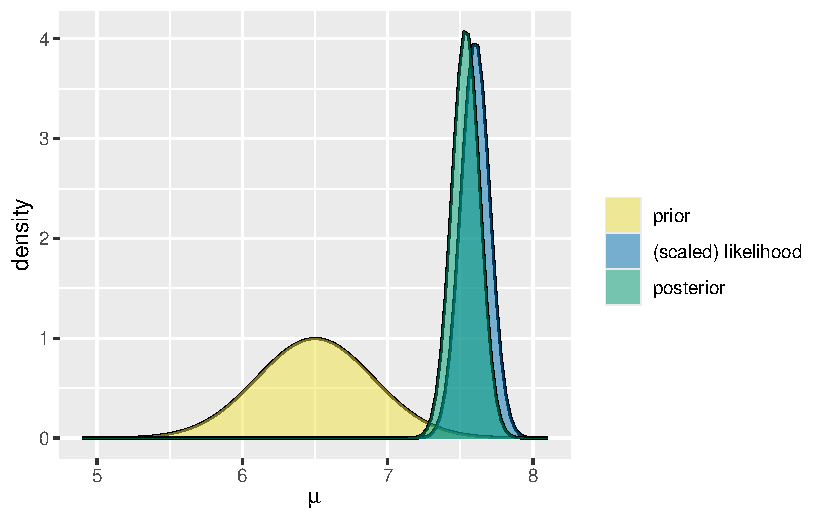
\includegraphics[keepaspectratio]{prueba_files/figure-pdf/unnamed-chunk-31-1.pdf}}

Nuevamente, dado que tenemos una verosimilitud cuyos datos estan tan
concentrados, el posterior se pega mucho a la verosimilitud, siendo
estos muy similares en forma y media.

\begin{longtable}[t]{lrrrr}
\caption{\label{tab:unnamed-chunk-33}Medidas de resumen para Normal-Normal(6.5, 0.4, 0.5, 7.6026, 25)}\\
\toprule
model & mean & mode & var & sd\\
\midrule
prior & 6.5000 & 6.5000 & 0.1600 & 0.400\\
posterior & 7.5377 & 7.5377 & 0.0094 & 0.097\\
\bottomrule
\end{longtable}

De esta manera confirmamos que nuestrio posterior calculado manualmente
en la Parte 2 era correcto.

\subsubsection{Ejercicio Normal-Normal
Conjugada}\label{ejercicio-normal-normal-conjugada}

\textbf{Consigna:}

\begin{enumerate}
\def\labelenumi{(\roman{enumi})}
\item
  Calcular la distribución a posteriori para μ.
\item
  Demostrar que la distribución a posteriori para μ es normal con media
  igual a un promedio ponderado de la media a priori θ y de la media
  muestral.
\item
  Analizar la influencia del tamaño muestral n sobre la media y la
  varianza de la distribución a posterior para μ. Conclusión: la
  distribución a priori normal para μ es conjugada con el modelo
  muestral de observaciones independientes de una población normal con
  media μ y varianza conocida σ2
\end{enumerate}

\textbf{Respuestas:} Nos basamos en la guia del libro para demostrar la
consigna paso a paso. Vamos a probar que la posteriori del modelo
Normal-Normal sigue tambien una distribucion normal

Primero, tenemos que la funcion de densidad de mu (posteriori) es
proporcional al producto de la funcion de densidad priori de la Normal y
la funcion de verosimilitud. Lo que queremos encontrar es la posteriori,
por otro lado, el priori es lo que sabiamos de mu antes de ver los datos
(la verosimilitud). Para todo mu perteneciente a los reales tenemos:

\[
\begin{aligned}
f(\mu|\vec{y}) &\propto f(\mu)L(\mu|\vec{y}) \propto \exp\left[-\frac{(\mu-\theta)^2}{2\tau^2}\right] \cdot \exp\left[-\frac{(\bar{y}-\mu)^2}{2\sigma^2/n}\right] \\[2ex]
\end{aligned}
\]

De forma resumida:

\[
\begin{align*}
f(\mu|\vec{y}) \propto \underbrace{\exp\left[-\frac{(\mu-\theta)^2}{2\tau^2}\right]}_{\text{Nucleo del Prior}} \cdot \underbrace{\exp\left[-\frac{(\bar{y}-\mu)^2}{2\sigma^2/n}\right]}_{\text{Nucleo de la Verosimilitud}}
\end{align*}
\]

El objetivo ahora es deshacernos de los paréntesis al cuadrado para
poder agrupar los términos que contienen \(\mu\). Para esto, se usa la
fórmula del binomio conjugado: \((a-b)^2 = a^2 - 2ab + b^2\).

Al expandir los exponentes, obtenemos:

\(-(\mu - \theta)^2 = -(\mu^2 - 2\mu\theta + \theta^2) = -\mu^2 + 2\mu\theta - \theta^2\)
\(-(\bar{y} - \mu)^2 = -(\mu - \bar{y})^2 = -(\mu^2 - 2\mu\bar{y} + \bar{y}^2) = -\mu^2 + 2\mu\bar{y} - \bar{y}^2\)

\[
\begin{aligned}
f(\mu|\vec{y}) &\propto \exp\left[\frac{-\mu^2 + 2\mu\theta - \theta^2}{2\tau^2}\right] \exp\left[\frac{-\mu^2 + 2\mu\bar{y} - \bar{y}^2}{2\sigma^2/n}\right] \\
\end{aligned}
\] Este siguiente paso es muy importante: ``nos olvidaremos de las
constantes''. Como estamos trabajando con proporcionalidad con respecto
a \(\mu\) y los terminos \(\theta^2\) y \(\bar{y}^2\) no contienen
ningun \(\mu\), consideramos a estos como constantes. Esto va a
simplificar mucho las cuentas. Obtenemos:

\[
\begin{aligned}
&\propto \exp\left[\frac{-\mu^2 + 2\mu\theta}{2\tau^2}\right] \exp\left[\frac{-\mu^2 + 2\mu\bar{y}}{2\sigma^2/n}\right] \\[2ex]
\end{aligned}
\] A continuacion, hacemos denominador comun para luego poder aplicar
las propiedades de potencia y sumar los exponentes:

\[
\begin{aligned}
&\propto \exp\left[\frac{(-\mu^2 + 2\mu\theta)\sigma^2/n}{2\tau^2\sigma^2/n}\right] \exp\left[\frac{(-\mu^2 + 2\mu\bar{y})n\tau^2}{2\tau^2\sigma^2/n}\right] \\
&\propto \exp\left[\frac{(-\mu^2 + 2\mu\theta)\sigma^2 + (-\mu^2 + 2\mu\bar{y})n\tau^2}{2\tau^2\sigma^2}\right]
\end{aligned}
\]

Ahora, agrupamos los terminos mu y mu\^{}2 para simplificar:

\[
\begin{aligned}
f(\mu|\vec{y}) &\propto \exp\left[\frac{-\mu^2(n\tau^2 + \sigma^2) + 2\mu(\theta\sigma^2 + \bar{y}n\tau^2)}{2\tau^2\sigma^2}\right] \\
\end{aligned}
\]

Como podemos hacer para demostrar que lo que obtuvimos es una
distribucion normal? Debemos lograr de alguna manera ``hacer aparecer''
el nucleo de la Normal. Un truco importante que se utiliza es el
``completee the square'' (completar el cuadrado).

\[
\begin{aligned}
&\propto \exp\left[\frac{-\mu^2 + 2\mu\left(\frac{\theta\sigma^2 + \bar{y}n\tau^2}{n\tau^2 + \sigma^2}\right)}{2(\tau^2\sigma^2)/(n\tau^2 + \sigma^2)}\right] \\[3ex]
\end{aligned}
\]

Ahora podemos factorizar:

\[
\begin{aligned}
f(\mu|\vec{y}) &\propto \exp\left[-\frac{\left(\mu - \frac{\theta\sigma^2 + \bar{y}n\tau^2}{n\tau^2 + \sigma^2}\right)^2}{2(\tau^2\sigma^2)/(n\tau^2 + \sigma^2)}\right] \\[3ex]
\end{aligned}
\]

Obtenemos el nucleo de una funcion de densidad de una Normal para mu.
Utilizando esto podemos concluir que la distribucion queda de esta
forma:

\[
\begin{aligned}
\mu|\vec{y} &\sim N\left(\frac{\theta\sigma^2 + \bar{y}n\tau^2}{n\tau^2 + \sigma^2}, \frac{\tau^2\sigma^2}{n\tau^2 + \sigma^2}\right) \\[3ex]
\end{aligned}
\]

Por lo tanto, queda demostrado que la posteriori de una Normal-Normal
conjugada es tambien una Normal.

Podemos reorganizar la media de la posteriori para demostrar que es el
promedio ponderado de la media a priori de \(\mu\) (\(E(\mu) = \theta\))
y la media de la muestra de \(\bar{y}\):

\textbf{- El peso del prior depende de los datos}

\textbf{- El peso de los datos depende del prior y de la cantidad de
datos}

\[
\begin{aligned}
\frac{\theta\sigma^2 + \bar{y}n\tau^2}{n\tau^2 + \sigma^2} &= \theta\frac{\sigma^2}{n\tau^2 + \sigma^2} + \bar{y}\frac{n\tau^2}{n\tau^2 + \sigma^2}
\end{aligned}
\]

Obtenemos tambien que la varianza a posteriori obtiene informacion de la
variabilidad a priori de \(\tau\) y la variabilidad en los datos de
\(\sigma\). Ambos se ven afectados por el tamano de la muestra, n.

En primer lugar, a medida que n aumente, la media a posteriori toma una
ponderacion menos en la media a priori y mayor ponderacion en la media
de la muestra \(\bar{y}\). Tenemos entonces:

\[
  \begin{aligned}
  \frac{\sigma^2}{n\tau^2 + \sigma^2} \to 0 \quad \text{y} \quad \frac{n\tau^2}{n\tau^2 + \sigma^2} \to 1
  \end{aligned}
  \]

Luego, cuando n aumenta, la variana posteriori disminuye:

\[
\begin{aligned}
\frac{\tau^2\sigma^2}{n\tau^2 + \sigma^2} \to 0
\end{aligned}
\]

Esto significa que, a medida que obtenemos mayor cantidad de datos, la
certeza de la posterior con respecto a \(\mu\) aumenta y se vuelve mas
cercana a los valores de la informacion.




\end{document}
